\documentclass{standalone}
\usepackage{tikz}
\usetikzlibrary{patterns, positioning}


\begin{document}
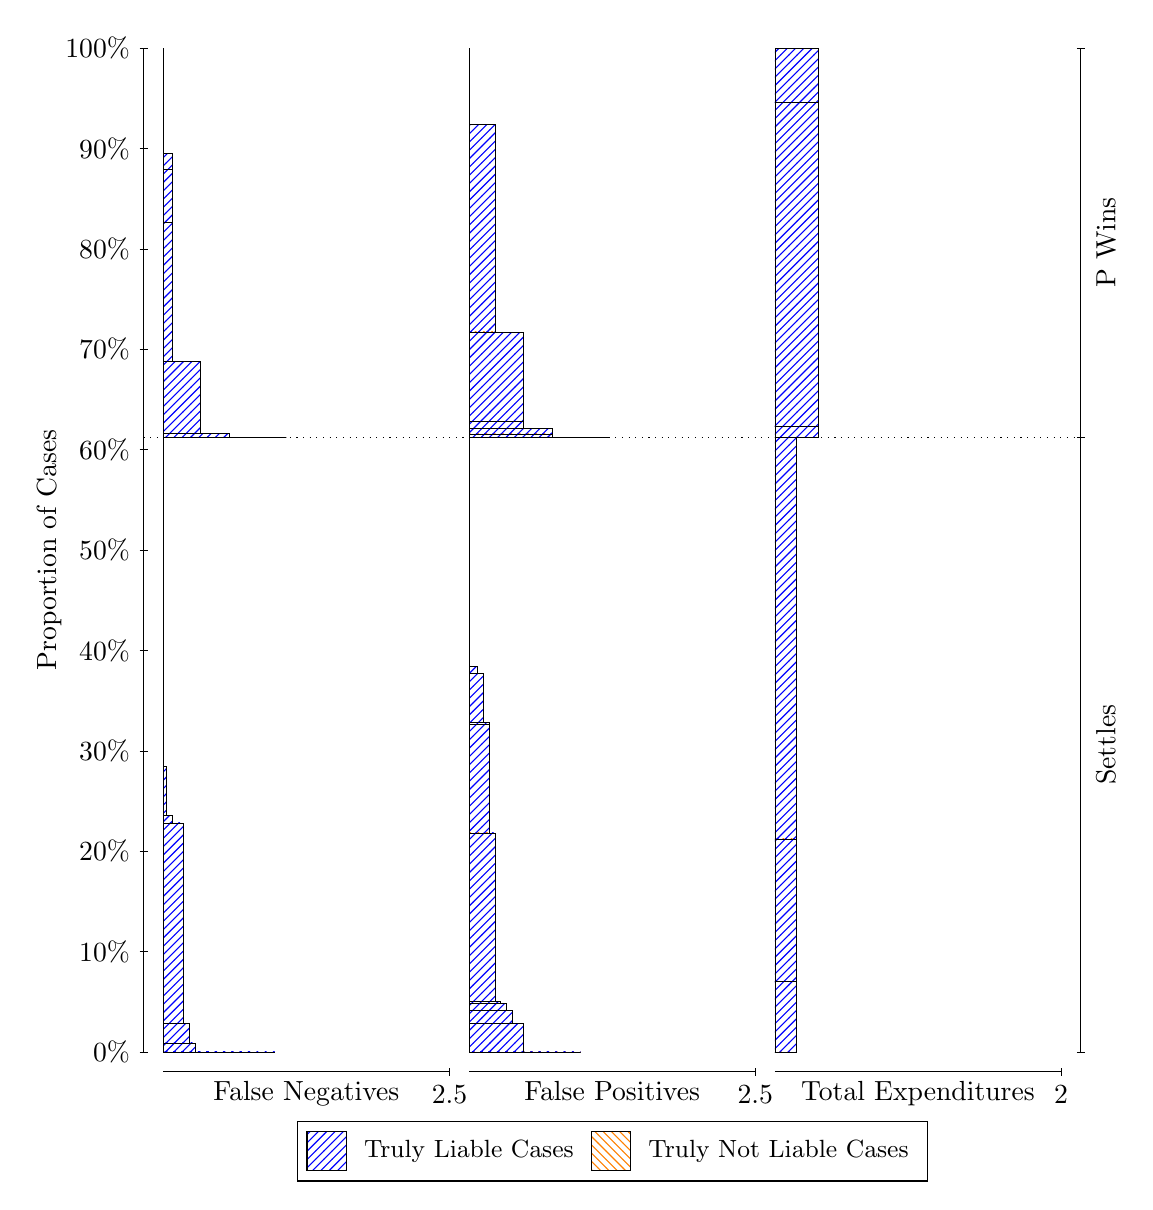
\begin{tikzpicture}
\draw[black, very thin] (1.5,1.75) -- (1.5,14.5);
\node[rotate=90, text=black, anchor=center] at (0.3, 8.125) {Proportion of Cases};
\draw[black, very thin] (1.45,1.75) -- (1.55,1.75);
\node[text=black, anchor=east] at (1.45, 1.75) {0\%};
\draw[black, very thin] (1.45,3.025) -- (1.55,3.025);
\node[text=black, anchor=east] at (1.45, 3.025) {10\%};
\draw[black, very thin] (1.45,4.3) -- (1.55,4.3);
\node[text=black, anchor=east] at (1.45, 4.3) {20\%};
\draw[black, very thin] (1.45,5.575) -- (1.55,5.575);
\node[text=black, anchor=east] at (1.45, 5.575) {30\%};
\draw[black, very thin] (1.45,6.85) -- (1.55,6.85);
\node[text=black, anchor=east] at (1.45, 6.85) {40\%};
\draw[black, very thin] (1.45,8.125) -- (1.55,8.125);
\node[text=black, anchor=east] at (1.45, 8.125) {50\%};
\draw[black, very thin] (1.45,9.4) -- (1.55,9.4);
\node[text=black, anchor=east] at (1.45, 9.4) {60\%};
\draw[black, very thin] (1.45,10.675) -- (1.55,10.675);
\node[text=black, anchor=east] at (1.45, 10.675) {70\%};
\draw[black, very thin] (1.45,11.95) -- (1.55,11.95);
\node[text=black, anchor=east] at (1.45, 11.95) {80\%};
\draw[black, very thin] (1.45,13.225) -- (1.55,13.225);
\node[text=black, anchor=east] at (1.45, 13.225) {90\%};
\draw[black, very thin] (1.45,14.5) -- (1.55,14.5);
\node[text=black, anchor=east] at (1.45, 14.5) {100\%};

\draw[black, very thin] (13.4,1.75) -- (13.4,14.5);
\draw[black, very thin] (13.35,1.75) -- (13.45,1.75);
\node[anchor=west] at (13.35, 1.75) {};
\draw[black, very thin] (13.35,9.5557) -- (13.45,9.5557);
\node[anchor=west] at (13.35, 9.5557) {};
\draw[black, very thin] (13.35,14.5) -- (13.45,14.5);
\node[anchor=west] at (13.35, 14.5) {};

\draw[black, very thin, pattern color=blue, pattern=north east lines] (1.75,1.75) rectangle (3.167,1.75);
\draw[black, very thin, pattern color=blue, pattern=north east lines] (1.75,1.75) rectangle (2.8763,1.75);
\draw[black, very thin, pattern color=blue, pattern=north east lines] (1.75,1.75) rectangle (2.8037,1.75);
\draw[black, very thin, pattern color=blue, pattern=north east lines] (1.75,1.75) rectangle (2.5857,1.75);
\draw[black, very thin, pattern color=blue, pattern=north east lines] (1.75,1.75) rectangle (2.513,1.7502);
\draw[black, very thin, pattern color=blue, pattern=north east lines] (1.75,1.7502) rectangle (2.4403,1.7513);
\draw[black, very thin, pattern color=blue, pattern=north east lines] (1.75,1.7513) rectangle (2.295,1.7513);
\draw[black, very thin, pattern color=blue, pattern=north east lines] (1.75,1.7513) rectangle (2.2223,1.7515);
\draw[black, very thin, pattern color=blue, pattern=north east lines] (1.75,1.7515) rectangle (2.1497,1.8656);
\draw[black, very thin, pattern color=blue, pattern=north east lines] (1.75,1.8656) rectangle (2.077,2.1129);
\draw[black, very thin, pattern color=blue, pattern=north east lines] (1.75,2.1129) rectangle (2.0043,4.6587);
\draw[black, very thin, pattern color=blue, pattern=north east lines] (1.75,4.6587) rectangle (1.9317,4.6597);
\draw[black, very thin, pattern color=blue, pattern=north east lines] (1.75,4.6597) rectangle (1.859,4.7513);
\draw[black, very thin, pattern color=blue, pattern=north east lines] (1.75,4.7513) rectangle (1.7863,5.3738);
\draw[black, very thin, pattern color=orange, pattern=north west lines] (1.75,5.3738) rectangle (1.75,5.3738);
\draw[black, very thin, pattern color=blue, pattern=north east lines] (1.75,5.3738) rectangle (1.75,9.5557);
\draw[black, very thin, pattern color=blue, pattern=north east lines] (1.75,9.5557) rectangle (3.3123,9.5557);
\draw[black, very thin, pattern color=blue, pattern=north east lines] (1.75,9.5557) rectangle (2.949,9.5558);
\draw[black, very thin, pattern color=blue, pattern=north east lines] (1.75,9.5558) rectangle (2.5857,9.6085);
\draw[black, very thin, pattern color=blue, pattern=north east lines] (1.75,9.6085) rectangle (2.2223,10.522);
\draw[black, very thin, pattern color=blue, pattern=north east lines] (1.75,10.522) rectangle (2.2223,10.524);
\draw[black, very thin, pattern color=blue, pattern=north east lines] (1.75,10.524) rectangle (1.859,12.288);
\draw[black, very thin, pattern color=blue, pattern=north east lines] (1.75,12.288) rectangle (1.859,12.957);
\draw[black, very thin, pattern color=blue, pattern=north east lines] (1.75,12.957) rectangle (1.859,13.165);
\draw[black, very thin, pattern color=orange, pattern=north west lines] (1.75,13.165) rectangle (1.75,13.165);
\draw[black, very thin, pattern color=blue, pattern=north east lines] (1.75,13.165) rectangle (1.75,14.5);
\draw[black, very thin, pattern color=orange, pattern=north west lines] (5.6333,1.75) rectangle (7.0503,1.75);
\draw[black, very thin, pattern color=blue, pattern=north east lines] (5.6333,1.75) rectangle (7.0503,1.75);
\draw[black, very thin, pattern color=orange, pattern=north west lines] (5.6333,1.75) rectangle (6.7597,1.75);
\draw[black, very thin, pattern color=blue, pattern=north east lines] (5.6333,1.75) rectangle (6.7597,1.75);
\draw[black, very thin, pattern color=blue, pattern=north east lines] (5.6333,1.75) rectangle (6.687,1.7513);
\draw[black, very thin, pattern color=orange, pattern=north west lines] (5.6333,1.7513) rectangle (6.6143,1.7513);
\draw[black, very thin, pattern color=blue, pattern=north east lines] (5.6333,1.7513) rectangle (6.6143,1.7513);
\draw[black, very thin, pattern color=orange, pattern=north west lines] (5.6333,1.7513) rectangle (6.469,1.7513);
\draw[black, very thin, pattern color=blue, pattern=north east lines] (5.6333,1.7513) rectangle (6.469,1.7516);
\draw[black, very thin, pattern color=blue, pattern=north east lines] (5.6333,1.7516) rectangle (6.3963,1.7524);
\draw[black, very thin, pattern color=blue, pattern=north east lines] (5.6333,1.7524) rectangle (6.3237,2.114);
\draw[black, very thin, pattern color=blue, pattern=north east lines] (5.6333,2.114) rectangle (6.251,2.1149);
\draw[black, very thin, pattern color=orange, pattern=north west lines] (5.6333,2.1149) rectangle (6.1783,2.1149);
\draw[black, very thin, pattern color=blue, pattern=north east lines] (5.6333,2.1149) rectangle (6.1783,2.2761);
\draw[black, very thin, pattern color=blue, pattern=north east lines] (5.6333,2.2761) rectangle (6.1057,2.368);
\draw[black, very thin, pattern color=blue, pattern=north east lines] (5.6333,2.368) rectangle (6.033,2.3892);
\draw[black, very thin, pattern color=blue, pattern=north east lines] (5.6333,2.3892) rectangle (5.9603,4.5322);
\draw[black, very thin, pattern color=orange, pattern=north west lines] (5.6333,4.5322) rectangle (5.8877,4.5322);
\draw[black, very thin, pattern color=blue, pattern=north east lines] (5.6333,4.5322) rectangle (5.8877,5.9105);
\draw[black, very thin, pattern color=blue, pattern=north east lines] (5.6333,5.9105) rectangle (5.8877,5.9319);
\draw[black, very thin, pattern color=blue, pattern=north east lines] (5.6333,5.9319) rectangle (5.815,6.5543);
\draw[black, very thin, pattern color=blue, pattern=north east lines] (5.6333,6.5543) rectangle (5.7423,6.646);
\draw[black, very thin, pattern color=blue, pattern=north east lines] (5.6333,6.646) rectangle (5.6697,6.647);
\draw[black, very thin, pattern color=blue, pattern=north east lines] (5.6333,6.647) rectangle (5.6333,9.5557);
\draw[black, very thin, pattern color=orange, pattern=north west lines] (5.6333,9.5557) rectangle (7.4137,9.5557);
\draw[black, very thin, pattern color=blue, pattern=north east lines] (5.6333,9.5557) rectangle (7.4137,9.5557);
\draw[black, very thin, pattern color=blue, pattern=north east lines] (5.6333,9.5557) rectangle (7.0503,9.5564);
\draw[black, very thin, pattern color=orange, pattern=north west lines] (5.6333,9.5564) rectangle (7.0503,9.5564);
\draw[black, very thin, pattern color=blue, pattern=north east lines] (5.6333,9.5564) rectangle (7.0503,9.5569);
\draw[black, very thin, pattern color=blue, pattern=north east lines] (5.6333,9.5569) rectangle (6.687,9.6003);
\draw[black, very thin, pattern color=orange, pattern=north west lines] (5.6333,9.6003) rectangle (6.687,9.6003);
\draw[black, very thin, pattern color=blue, pattern=north east lines] (5.6333,9.6003) rectangle (6.687,9.6667);
\draw[black, very thin, pattern color=blue, pattern=north east lines] (5.6333,9.6667) rectangle (6.3237,9.7618);
\draw[black, very thin, pattern color=orange, pattern=north west lines] (5.6333,9.7618) rectangle (6.3237,9.7618);
\draw[black, very thin, pattern color=blue, pattern=north east lines] (5.6333,9.7618) rectangle (6.3237,10.891);
\draw[black, very thin, pattern color=blue, pattern=north east lines] (5.6333,10.891) rectangle (5.9603,10.894);
\draw[black, very thin, pattern color=orange, pattern=north west lines] (5.6333,10.894) rectangle (5.9603,10.894);
\draw[black, very thin, pattern color=blue, pattern=north east lines] (5.6333,10.894) rectangle (5.9603,13.532);
\draw[black, very thin, pattern color=blue, pattern=north east lines] (5.6333,13.532) rectangle (5.6333,14.5);
\draw[black, very thin, pattern color=orange, pattern=north west lines] (9.5167,1.75) rectangle (9.7892,1.75);
\draw[black, very thin, pattern color=blue, pattern=north east lines] (9.5167,1.75) rectangle (9.7892,2.6478);
\draw[black, very thin, pattern color=orange, pattern=north west lines] (9.5167,2.6478) rectangle (9.7892,2.6478);
\draw[black, very thin, pattern color=blue, pattern=north east lines] (9.5167,2.6478) rectangle (9.7892,4.4576);
\draw[black, very thin, pattern color=orange, pattern=north west lines] (9.5167,4.4576) rectangle (9.7892,4.4576);
\draw[black, very thin, pattern color=blue, pattern=north east lines] (9.5167,4.4576) rectangle (9.7892,9.5557);
\draw[black, very thin, pattern color=orange, pattern=north west lines] (9.5167,9.5557) rectangle (10.062,9.5557);
\draw[black, very thin, pattern color=blue, pattern=north east lines] (9.5167,9.5557) rectangle (10.062,9.6975);
\draw[black, very thin, pattern color=orange, pattern=north west lines] (9.5167,9.6975) rectangle (10.062,9.6975);
\draw[black, very thin, pattern color=blue, pattern=north east lines] (9.5167,9.6975) rectangle (10.062,13.811);
\draw[black, very thin, pattern color=orange, pattern=north west lines] (9.5167,13.811) rectangle (10.062,13.811);
\draw[black, very thin, pattern color=blue, pattern=north east lines] (9.5167,13.811) rectangle (10.062,14.5);
\draw[black, dotted] (1.5,9.5557) -- (13.4,9.5557);
\draw[black, very thin] (1.75,1.5) -- (5.3833,1.5);
\node[text=black, anchor=north] at (3.5667, 1.5) {False Negatives};
\draw[black, very thin] (5.3833,1.45) -- (5.3833,1.55);
\node[text=black, anchor=north] at (5.3833, 1.45) {2.5};

\draw[black, very thin] (5.6333,1.5) -- (9.2667,1.5);
\node[text=black, anchor=north] at (7.45, 1.5) {False Positives};
\draw[black, very thin] (9.2667,1.45) -- (9.2667,1.55);
\node[text=black, anchor=north] at (9.2667, 1.45) {2.5};

\draw[black, very thin] (9.5167,1.5) -- (13.15,1.5);
\node[text=black, anchor=north] at (11.333, 1.5) {Total Expenditures};
\draw[black, very thin] (13.15,1.45) -- (13.15,1.55);
\node[text=black, anchor=north] at (13.15, 1.45) {2};

\node[text=black, centered, rotate=90] at (13.72, 5.6528) {Settles};
\node[text=black, centered, rotate=90] at (13.72, 12.028) {P Wins};

\draw (7.449999999999999,1.5) node[draw=none] (baseCoordinate) {};
\begin{scope}[align=center]
        \matrix[scale=0.5, draw=black, below=0.5cm of baseCoordinate, nodes={draw}, column sep=0.1cm]{
            \node[rectangle, draw, minimum width=0.5cm, minimum height=0.5cm, pattern color=blue, pattern=north east lines] {}; &
            \node[draw=none, font=\small, text=black] (B) {Truly Liable Cases}; &
            \node[rectangle, draw, minimum width=0.5cm, minimum height=0.5cm, pattern color=orange, pattern=north west lines] {}; &
            \node[draw=none, font=\small, text=black] (B) {Truly Not Liable Cases}; \\
            };
\end{scope}

\end{tikzpicture}
\end{document}